\documentclass[10pt,a4paper]{article}
\usepackage[utf8]{inputenc}

% Define the page margin
\usepackage[margin=3cm]{geometry}

% Better typography (font rendering)
\usepackage{microtype}

% Math environments and macros
\usepackage{amsmath}
\usepackage{amsfonts}
\usepackage{amssymb}
\usepackage{amsthm}

% Define \includegraphics to include graphics
\usepackage{graphicx}

% Draw graphics from a text description
\usepackage{tikz}

% Syntax highlighting
\usepackage{minted}

% Set global minted options
\setminted{linenos, autogobble, frame=lines, framesep=2mm}

% Import the comment environment for orgtbl-mode
\usepackage{comment}

% Do not indent paragraphs
\usepackage{parskip}

\title{Operating Systems, Sheet 6}
\author{Marten Lienen (03670270)}

\begin{document}

\maketitle

\section*{Exercise 1}

\subsection*{Part 1.1)}

\subsubsection*{Part 1)}

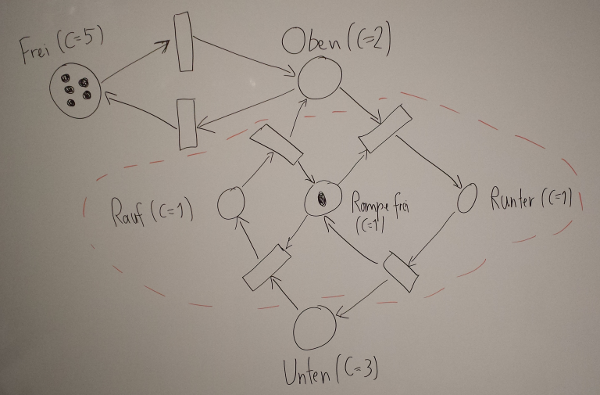
\includegraphics[width=\textwidth]{sheet-6/exercise-1-1-1}

\subsubsection*{Part 2)}

Der kritische Bereich ist rot umrandet.

\subsection*{Part 1.2)}

\subsubsection*{Part 1)}

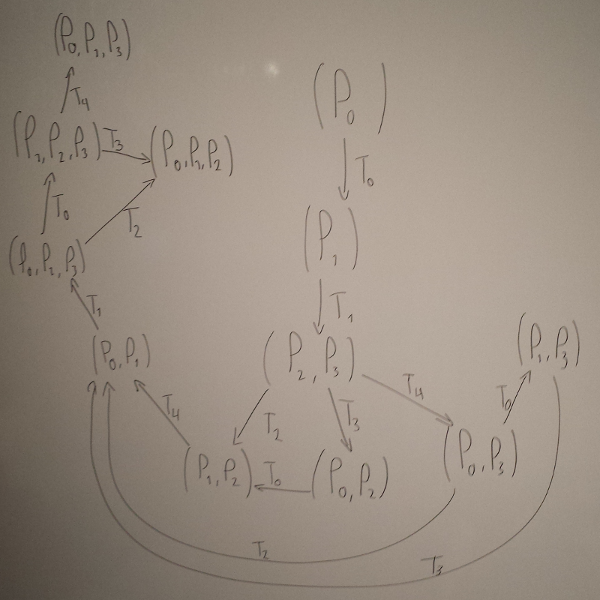
\includegraphics[width=\textwidth]{sheet-6/exercise-1-2-1}

\subsubsection*{Part 2)}

Das Netz ist verklemmt, weil es von den zwei Knoten $(P_{0}, P_{1}, P_{2})$ und $(P_{0}, P_{1}, P_{3})$ keine Kante wegführt.
Ein anderer Weg dies einzusehen ist, dass es ein Netz mit endlichen Kapazitäten und einer Markenquelle aber ohne Markensenke ist.

\subsubsection*{Part 3)}

Wie in Teil 2 begründet, müssen wir eine Markensenke einführen.
Dazu führen wir eine neue Stelle $P_{4}$ ein und eine Transition $T_{5}$, die Marken mit $(P_{0}, P_{1}) \rightarrow (P_{4})$ verschiebt.
Dies führt von den verklemmten Konfigurationen zu $(P_{2}, P_{4})$ bzw. $(P_{3}, P_{4})$.
Um von dort weg zu kommen brauchen wir noch eine letzte Transition $T_{6}$ definiert durch $(P_{4}) \rightarrow (P_{0})$.
Diese überführt die neuen Knoten im Erreichbarkeitsgraph in bereits existierenden Knoten $(P_{0}, P_{2})$ und $(P_{0}, P_{3})$.

\section*{Exercise 2}

\begin{itemize}
\item notify wakes one suspended thread whereas notifyAll wakes all of them.
\item Thread Interference tritt auf, wenn die Ausführung von Threads auf eine Art überlappt, in der das Endergebnis nicht \emph{einer} sequentiellen Ausführung entspricht.
  Bei Memory Consistency Errors wird das versprochene Konsistenzmodell des Speichers verletzt.
  Das heißt beispielsweise, dass Threads Werte im Speicher in unterschiedlicher Reihenfolge sehen.
\item happenedBefore ist wie in Distributed Systems
\item Jedes Objekt in Java hat ein Lock mit sich assoziiert, dass benutzt werden kann, wenn mehrere Threads nebenläufig auf Eigenschaften dieses Objekts zugreifen, und \emph{intrinsic lock} oder \emph{monitor lock} genannt wird
\item Mit wait wartet ein Thread darauf, dass ein anderer Thread ihn aufweckt, und mit notify tut man genau dies.
  So implementiert man das Warten auf das Eintreten einer bestimmten Bedingung wie z.B. das Vorhandensein von Elementen in einer Queue
\end{itemize}

\begin{minted}{java}
  public class Semaphor {
    private int level;

    public Semaphor(int level) {
      this.level = level;
    }

    public synchronized void V() {
      this.level++;
      this.notifyAll();
    }

    public synchronized void P() {
      while (this.level < 1) {
        try {
          this.wait();
        } catch (InterruptedException e) {
          // Recheck condition
        }
      }

      this.level--;
    }
  }
\end{minted}

\section*{Exercise 3}

\inputminted{c}{sheet-6/fabrik.c}

\end{document}
